\section{A Reproducible Intervention-Conditioned Response}
\label{sec:repro}

We first establish that the outcome used for mechanism discrimination is not a
single-checkpoint or single-run accident. This section is an empirical base for
the functional-damage question; it is not presented as discovery of the broad
training phenomenon.

\begin{table}[t]
\centering
\scriptsize
\caption{Selected validated results. Intervals bootstrap independent-run summaries.}
\begin{tabular}{@{}p{0.29\columnwidth}p{0.43\columnwidth}p{0.15\columnwidth}@{}}
\toprule
Result & Estimate & Replicates \\
\midrule
WikiText-2 $\deltas$ & $-0.1035$ [$-0.1115,-0.0958$] & 9/9 \\
HellaSwag $\deltas$ & $-0.0793$ [$-0.0885,-0.0677$] & 6/6 \\
Magnitude-matched contrast & $+0.0430$ [$0.0354,0.0525$] & 6/6 \\
Damage-matched contrast & $+0.0025$ [$-0.0009,0.0058$] & 4/6 \\
Corrected family residual & $-0.0168$ [$-0.0200,-0.0126$] & 5/5 \\
Geometry-adjusted residual & $-0.0134$ [$-0.0176,-0.0092$] & 5 runs \\
\bottomrule
\end{tabular}
\label{tab:key-results}
\end{table}


\paragraph{Independent runs and held-out prediction.}
Across nine independent 160M pretraining runs, every late-minus-early
block-bypass change is negative. Mean $\deltas$ is $-0.10353$, with a
run-bootstrap 95\% interval $[-0.11149,-0.09585]$; the median is $-0.10410$.
Run 9 was prospectively held out before its weights were evaluated. Its
$\deltas=-0.11895$ has the predicted sign and lies inside the frozen prediction
interval $[-0.13463,-0.06366]$. Intact NLL improves from an early-run mean of
3.878 to a late-run mean of 3.726, so the endpoint is not explained by a failure
to learn next-token prediction.

The direction is broad across the tested locations: all 90 run--interior-layer
endpoint changes are negative, and all ten layer medians are negative. The
magnitude is not uniform; layer medians range from $-0.0653$ to $-0.1838$.
Accordingly, we claim broad sign support, not location invariance.

\paragraph{Confidence control.}
Top-1 agreement is mechanically related to intact confidence. We therefore
repeat the endpoint comparison within five fixed intact-confidence bins. All
45 eligible run--bin changes are negative, with mean matched change $-0.11388$.
This control conditions on a coarse observable and does not fully match token
difficulty.

\paragraph{Scale and corpus boundaries.}
Five independent 70M runs reproduce the direction (5/5 negative; median
$\deltas=-0.14334$, 95\% interval $[-0.15385,-0.11030]$). This is replication at
two small scales inside one architecture family, not a scaling law.

On the HellaSwag-derived stream, all six 160M runs are negative, with mean
$\deltas=-0.07926$ and 95\% interval $[-0.08851,-0.06767]$. All 30 confidence-
bin changes are also negative. The absolute effect is 0.766 times the
WikiText-2 mean (95\% interval $[0.645,0.880]$): the direction repeats but the
magnitude is corpus-dependent. HellaSwag is easier and more confident under the
frozen stream, so the comparison does not imply corpus invariance.

\begin{figure*}[t]
\centering
\begin{minipage}[t]{0.32\textwidth}\centering
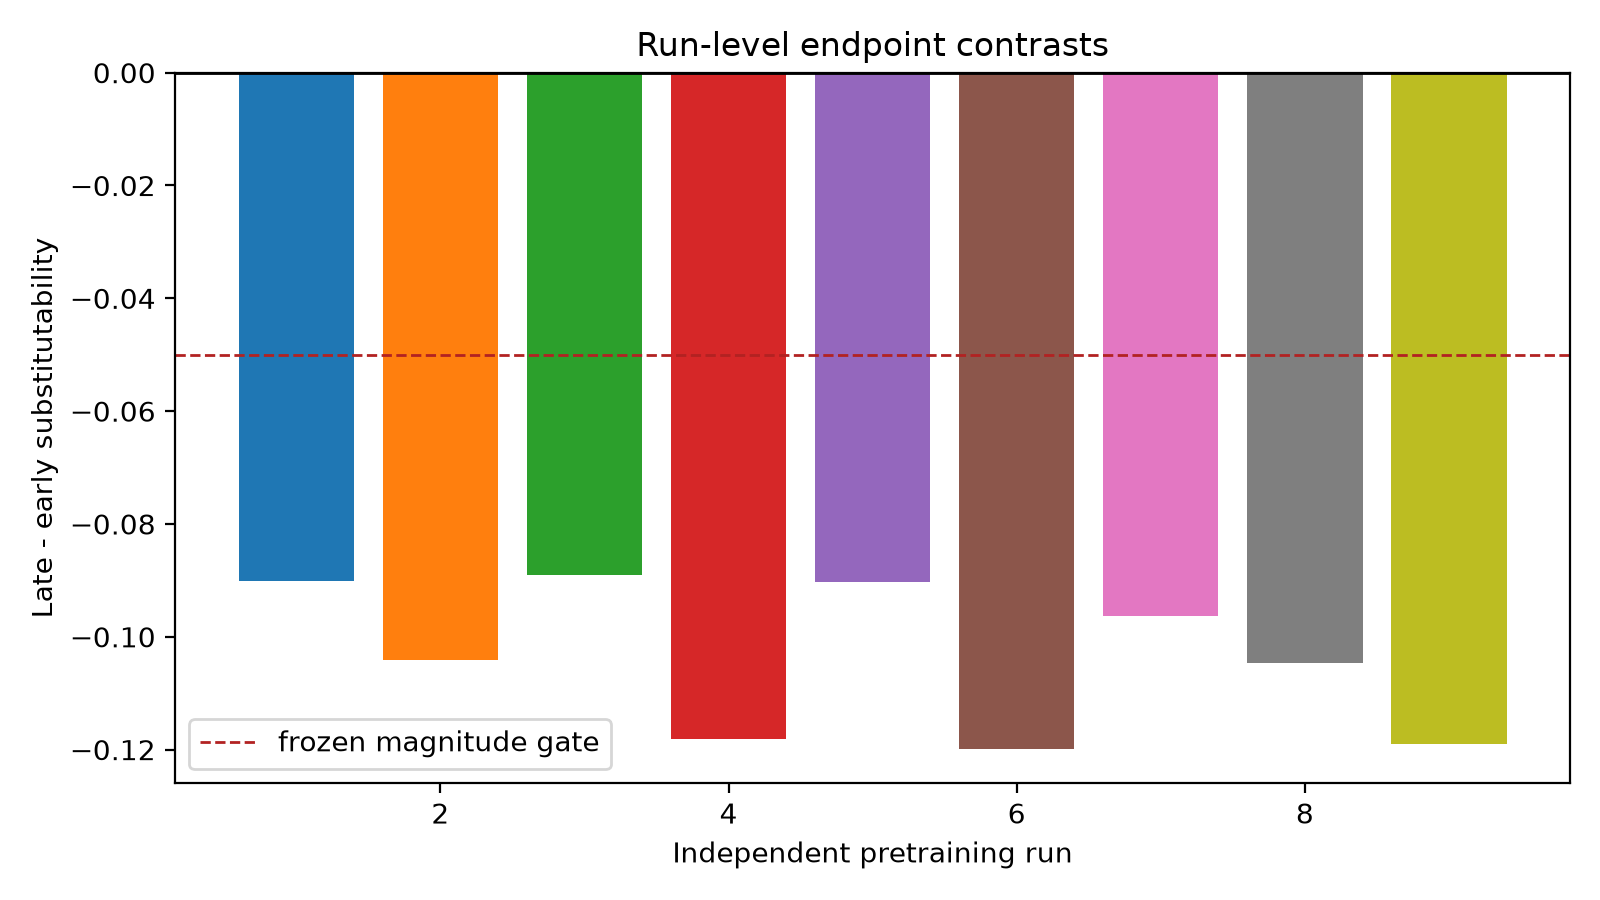
\includegraphics[width=\linewidth]{figures/draft2/fig1_pythia160.png}
\\[-2mm]\small (a) Nine independent 160M runs
\end{minipage}\hfill
\begin{minipage}[t]{0.32\textwidth}\centering
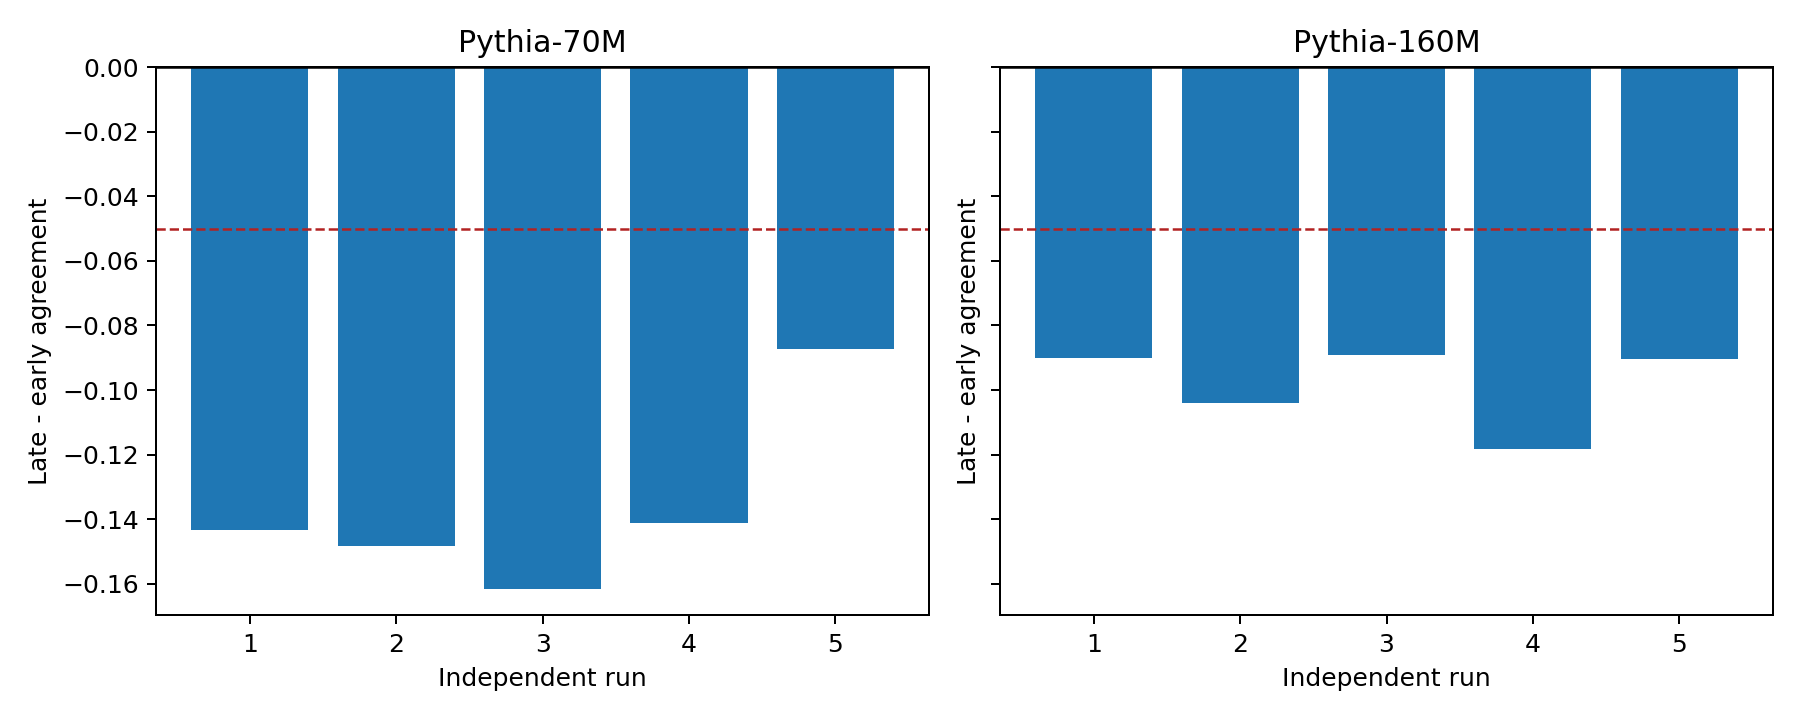
\includegraphics[width=\linewidth]{figures/draft2/fig1_pythia70.png}
\\[-2mm]\small (b) Five independent 70M runs
\end{minipage}\hfill
\begin{minipage}[t]{0.32\textwidth}\centering
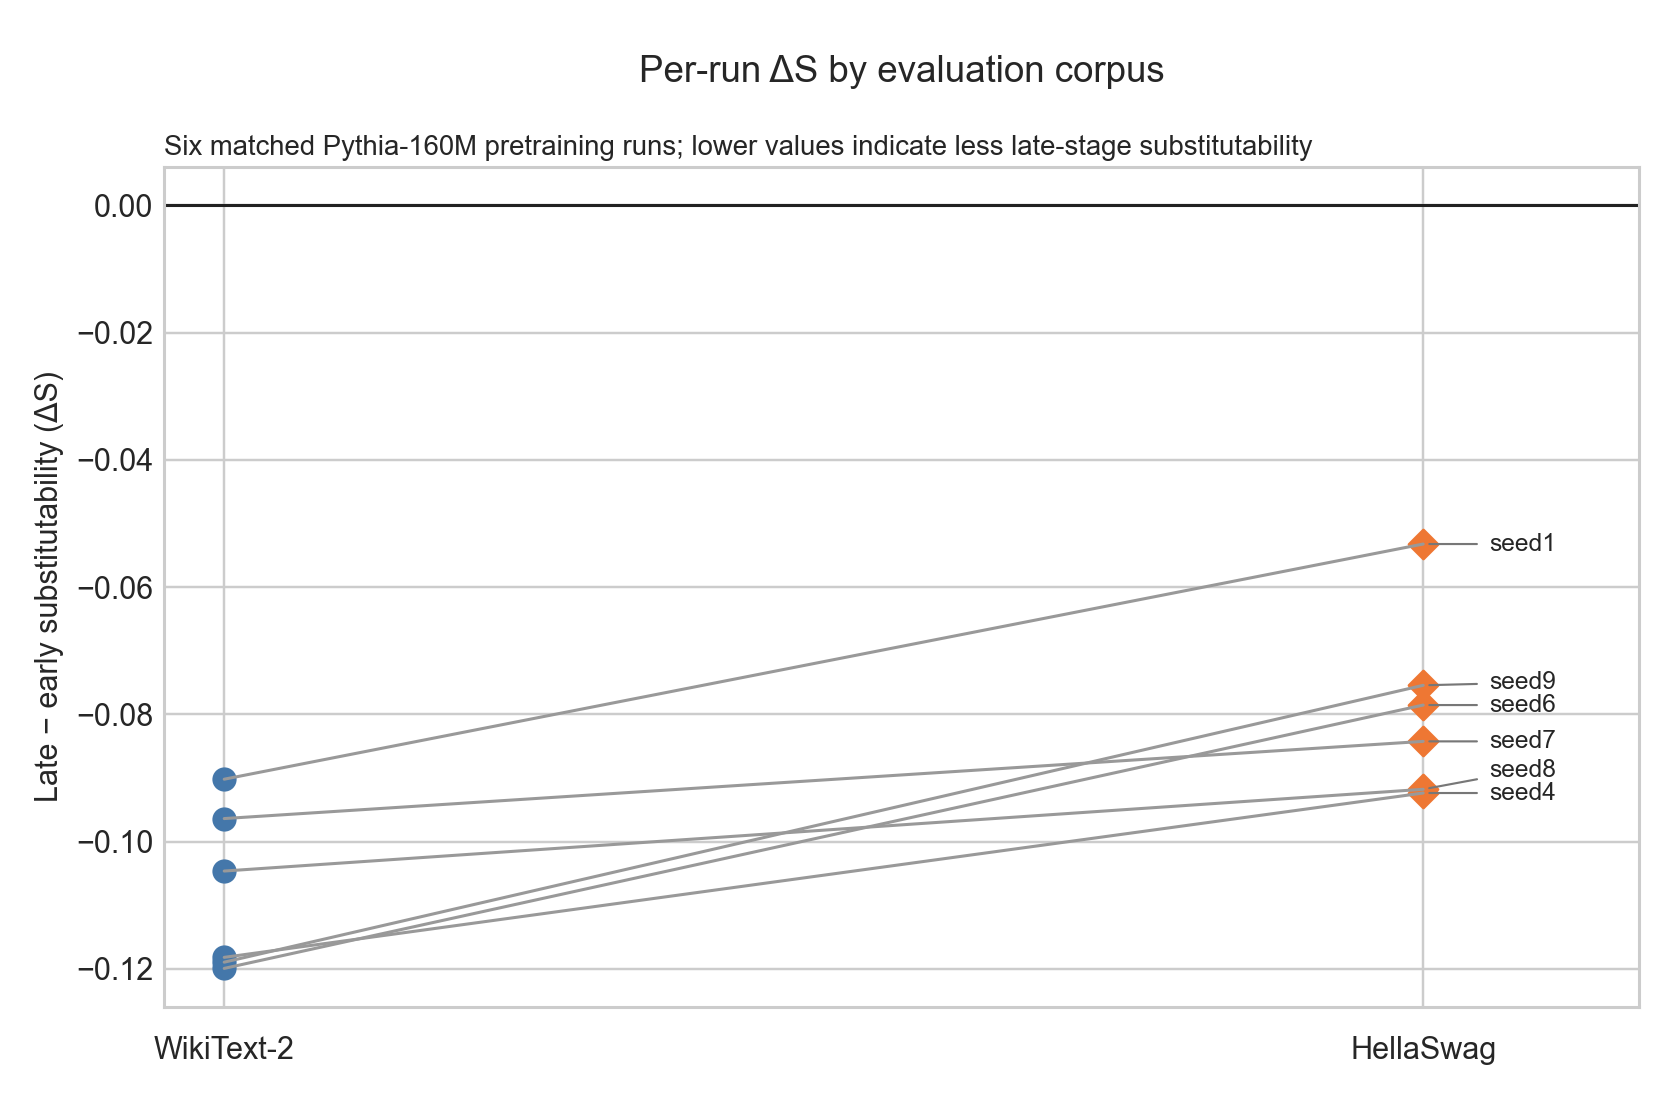
\includegraphics[width=\linewidth]{figures/draft2/fig1_hellaswag.png}
\\[-2mm]\small (c) HellaSwag-derived stream
\end{minipage}
\caption{\textbf{Empirical base.} The endpoint direction repeats across
independent runs, two small scales, and two evaluation streams. Panels reuse
sealed ARC figures without recomputing outcomes. Differences in magnitude are
not interpreted as invariance or a scaling law.}
\label{fig:repro}
\end{figure*}

Taken together, these checks justify using the endpoint response as a stable
outcome for the controlled comparisons that follow. They do not establish why
the response changes.
